
% Definir nova margem só para a frontpage
\newgeometry{margin=2cm}

\begin{titlepage}

% centrar tudo
\centering

% Imagem + titulo do trabalho
\begin{tikzpicture}
\node[inner sep=0pt] (logo) at (0,0.65)
    {
\includegraphics[scale=0.75]{Figures/0. General/atec_2.png}};
{\setstretch{1.75}
\node[text width = 0.38\textwidth, yshift = 0.35cm, right = 1.25cm of logo](title){\sffamily\huge\reporttitle};
}   
\node[text width = 0.5\textwidth, xshift = 0.92cm, yshift = 0.5cm, below = 0.5cm of title](subtitle){\sffamily\large\reportsubtitle};
\gettikzxy{(subtitle.south)}{\sffamily\subtitlex}{\subtitley}
\gettikzxy{(title.north)}{\titlex}{\titley}
\draw[line width=1.75mm, color_scheme]($(logo.east)!0.5!(title.west)$) +(0,\subtitley - 0.69cm) -- +(0,\titley - 0.96cm);
\end{tikzpicture}

\vspace{0.5cm}

% reduzir horizontalmente a largura para criar enfase visual
\setlength{\hsize}{0.9\hsize}

% Curso
\hspace{0.75cm}\footnotesize \textbf{\cursoextenso ~-~\curso} \\

% Espaço em branco no centro
\vspace{5.5cm}

% logotipo
\makebox[0.85\textwidth][r]{
\includegraphics[scale=1.5]{Figures/0. General/hidden_solutions.jpg}}

% Espaço em branco no centro
\vspace{3cm}

% Autores e formador
\begin{tikzpicture}
    \setstretch{1.2} \node[text width = 0.23\textwidth] (autores) at (0,0) {\sffamily\large\autores};
    \hspace{2cm}\node[text width = 0.23\textwidth, yshift=0.95cm, right = 7.5cm of autores](formador) at (0,0){\sffamily\large\formador};
\end{tikzpicture}

% Imagem da ATEC
\tikz[remember picture,overlay]\node[anchor=south,inner sep=0pt] at (current page.south) {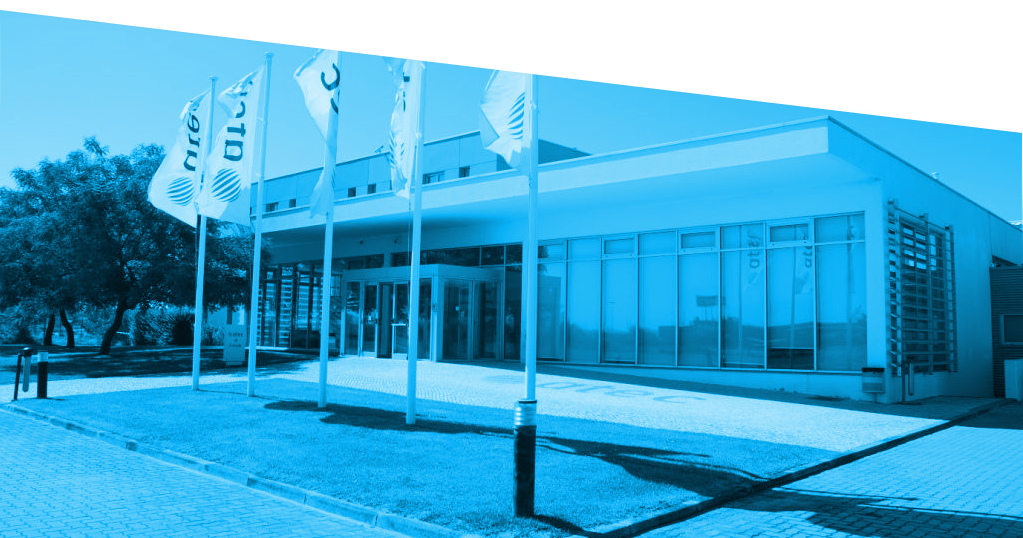
\includegraphics[width=\paperwidth]{Figures/0. General/atec.png}};
\mbox{}
\vfill
\begin{figure}[H]
    \centering
    \hspace{-0.35cm}
    \vspace{-0.5cm}
    % width=\textwidth para imagem da largura do texto
    
\includegraphics[scale=0.5]{Figures/0. General/atec_logo_white.png}
\end{figure}

% Local e data
\hspace{1.27cm} \sffamily \LARGE \textcolor{white}{\placeanddate}\\

\end{titlepage}

% Restore the original geometry
\restoregeometry







